Per valutare l'andamento dell'RTT minimo, medio, massimo e della deviazione standard in funzione della dimensione del pacchetto abbiamo creato uno script bash "ping\_rtt.sh". Questo script automatizza il processo di esecuzione del comando \texttt{ping} con diverse dimensioni del pacchetto e raccoglie i valori di RTT corrispondenti.\\\\
Lo script utilizza un ciclo \texttt{for} per iterare attraverso una serie di dimensioni del pacchetto. Per ogni dimensione del pacchetto, esegue il comando ping specificando il numero di pacchetti da inviare e la dimensione del payload del pacchetto.\\ Successivamente, estrae l'ultima linea di output del comando ping, che contiene i valori di RTT minimo, medio, massimo e deviazione standard. Questi valori vengono salvati in un file di testo in un formato conveniente per l'acquisizione dei dati da parte di MATLAB \Rcerchio.\\\\
Nel test, abbiamo scelto di inviare per ogni dimensione del pacchetto $K=100$ pacchetti per avere una valutazione migliore delle statistiche dell' RTT. La dimensione dei pacchetti è variabile da 10 a 1472 byte con passi di 1 byte. Questa scelta ci consente di ottenere una rappresentazione dettagliata dell'andamento dell'RTT in base alla dimensione del pacchetto.\\\\
Si è scritto un programma MATLAB \Rcerchio che legge i dati dal file e genera un semplice grafico dei valori di RTT in funzione della dimensione del pacchetto. Abbiamo riportato in Figura \ref{fig:risRTT} i risultati.
\section{Stima di \textit{R} e \textit{R-bottleneck}}
Sappiamo che generalmente l'RTT aumenta con la lunghezza dei pacchetti, nella pratica questa regolazione può essere influenzata dalla variabilità del ritardo di accodamento. Considerando il valore minimo dell'RTT possiamo mitigare l'effetto dei ritardi di accodamento, misurato su una serie di trasmissioni con pacchetti di dimensione costante. Infatti si ipotizza che prima o poi il pacchetto possa trovare tutte le code vuote ad ogni nodo. In formule, assumeremo che, eseguendo un numero $K$ sufficientemente grande di volte il \texttt{ping} con $L$ costante, si abbia:
\begin{equation}
    RTT_{\min}(L)\approx aL+T
\end{equation}
In effetti, come osservato dalla Figura \ref{fig:risR} è evidente che l'andamento del minimo dell'RTT per ogni valore di $L$ è stato ben approssimato linearmente da una retta. La linearità dell'andamento del minimo dell'RTT implica che all'aumentare della dimensione dei pacchetti, il tempo di trasmissione minimo aumenta proporzionalmente.
\begin{figure}[H]
    \centering
    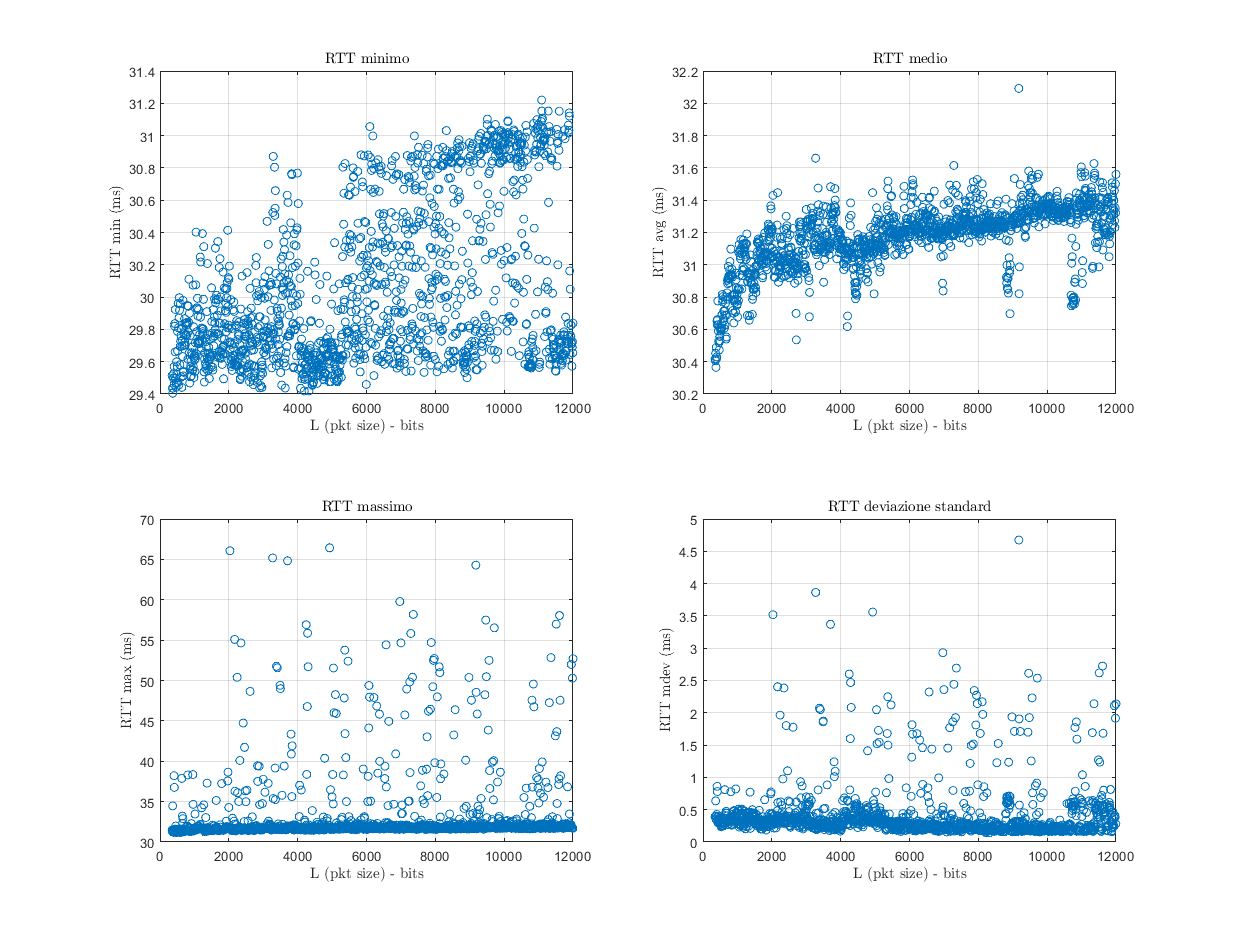
\includegraphics[width=\linewidth]{rtt all.png}
    \caption{Statistiche dell'RTT in funzione della dimensione del pacchetto}
    \label{fig:risRTT}
\end{figure}
\begin{figure}[H]
    \centering
    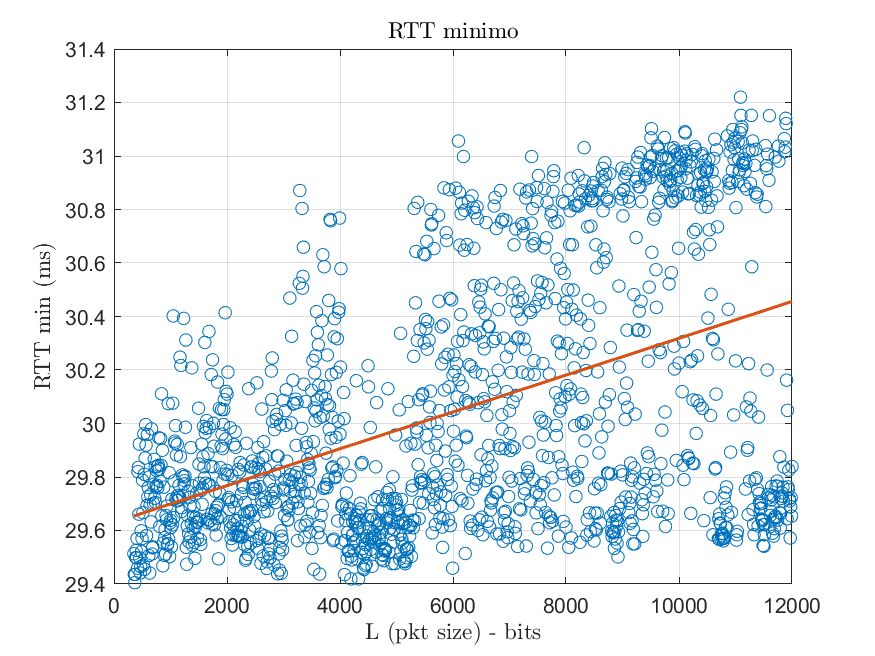
\includegraphics[width=\linewidth]{rtt fit.png}
    \caption{Statistiche dell'RTT minimo in funzione della dimensione del pacchetto con curva di andamento}
    \label{fig:risR}
\end{figure}
Stimando la pendenza della retta che approssima l'andamento del minimo dell'RTT in funzione delle dimensioni dei pacchetti, possiamo ottenere una stima del coefficiente $a$. Questo coefficiente ci fornisce informazioni utili per valutare il throughput della rete in due diverse ipotesi:
\begin{itemize}
    \item Se tutti i link (andata e ritorno) hanno throughput uguali ad un certo valore $R$, si ottiene
    \begin{equation}
        R=\frac n a
    \end{equation}
    \item Se invece esiste un link con un throughput molto minore di tutti gli altri (detto \textit{bottleneck}), e supponendo che tale throughput sia lo stesso all’andata ed al ritorno si ha:
    \begin{equation}
        R_{\text{bottleneck}}\approx \frac 2 a
    \end{equation}
\end{itemize}
\clearpage
È importante sottolineare che queste stime sono basate sulle ipotesi semplificate sull'omogeneità dei link e sulla simmetria del throughput nel caso del bottleneck. Sappiamo dalle stime fatte al punto \ref{ch:link} che il server \texttt{"lon.speedtest.clouvider.net"} ha $n=11*2=22$ pertanto otteniamo:
\begin{equation*}
    a=6.8818\cdot10^{-5}\quad R=319.6849\text{ kbps}\quad R_{\text{bottleneck}}=29.0623\text{ kbps}
\end{equation*}
\section{Conclusioni}
Attraverso l'utilizzo dell' applicazione \texttt{ping} e l'analisi dei valori di RTT siamo stati in grado di apprezzare l'andamento dell'RTT in relazione alla dimensione dei pacchetti, riusciendo a mitigare l'impatto dei ritardi di accodamento sulla misurazione.\\\\
Abbiamo osservato che, sebbene l'RTT tendenzialmente cresca con la lunghezza dei pacchetti, questa relazione può essere influenzata dalla variabilità del ritardo di accodamento. Tuttavia, abbiamo dimostrato che considerando il valore minimo di RTT misurato su una serie di trasmissioni con pacchetti di dimensione costante, possiamo mitigare l'impatto dei ritardi di accodamento.\\\\
Abbiamo ripetuto l'esperimento anche con altri server: ottenendo prestazioni peggiori con server più lontani geograficamente.